\chapter{Implémentation et Déploiement}
\vspace{-1.5em}
\chaptertoc
\vspace{-2.5em}
\section{Introduction}
Ce chapitre présente les résultats obtenus à travers différentes métriques de performance, avant de traiter les aspects pratiques liés au déploiement du système ainsi que les interfaces développées pour en faciliter l’utilisation opérationnelle.
\vspace{-1.2em}
\section{Métriques d’Évaluation}
\vspace{-1em}
L’évaluation des performances des algorithmes d’affectation de stands nécessite un cadre d’analyse complet, intégrant à la fois l’efficacité opérationnelle et la performance algorithmique. Pour atteindre cet objectif, nous définissons deux catégories distinctes de métriques d’évaluation, offrant des perspectives complémentaires sur les performances des solutions proposées.

\subsection{Métriques de Validation des Performances}

La première catégorie regroupe des métriques visant à valider les performances de l’algorithme par rapport aux données opérationnelles réelles du \ac{SOAM}. Ces métriques mesurent à quel point les solutions générées par l’algorithme se rapprochent des décisions et contraintes opérationnelles.

\begin{enumerate}
	\item \textbf{Taux d’affectation des vols} : mesure le pourcentage de vols affectés avec succès à un stand, ce qui reflète la capacité de l’algorithme à gérer l’ensemble du programme de vols.
	\vspace{-1em}
	\begin{equation}
		\eta_{assigned} = \frac{|F_{assigned}|}{|F_{total}|} \times 100\%
	\end{equation}
	\vspace{-1em}
	\item \textbf{Taux de respect des contraintes} : évalue la proportion de contraintes opérationnelles respectées dans la solution finale, garantissant le respect des exigences de sécurité et d’exploitation.
	\vspace{-1em}
	\begin{equation}
		\gamma_{constraints} = \frac{|C_{satisfied}|}{|C_{total}|} \times 100\%
	\end{equation}
	
	\item \textbf{Utilisation des stands de contact} : quantifie l’efficacité d’utilisation des stands de contact, généralement préférés pour le confort des passagers.
	\vspace{-1em}
	\begin{equation}
		\rho_{contact} = \frac{|S_{contact}^{used}|}{|S_{contact}^{total}|} \times 100\%
	\end{equation}
	
	\item \textbf{Utilisation des stands éloignés} : mesure le taux d’utilisation des stands éloignés, fournissant une indication sur la répartition des ressources.
	\vspace{-0.7em}
	\begin{equation}
		\rho_{remote} = \frac{|S_{remote}^{used}|}{|S_{remote}^{total}|} \times 100\%
	\end{equation}
\end{enumerate}

\subsection{Métriques de Comparaison des algorithmes}

La seconde catégorie regroupe des métriques conçues pour comparer de manière systématique les performances relatives de différents algorithmes.

\begin{enumerate}
	\item \textbf{Stabilité des solutions} : évalue la régularité des résultats d’affectation sur plusieurs exécutions de l’algorithme avec les mêmes données d’entrée. Cette métrique est cruciale pour garantir que la solution finale soit fiable et réutilisable en environnement réel.
	\begin{equation}
		\sigma_{stable} = \frac{\text{Nombre d'affectations cohérentes}}{\text{Nombre total d'exécutions}} \times 100\%
	\end{equation}
	
	\item \textbf{Temps de calcul} : mesure la durée réelle d’exécution nécessaire pour obtenir une solution, indiquant l’adaptabilité de l’algorithme aux environnements en temps réel.
	\begin{equation}
		T_{exec} = t_{end} - t_{start}
	\end{equation}
	
	\item \textbf{Complexité temporelle} : représente la complexité computationnelle théorique de l’algorithme en fonction de la taille du problème.
	\vspace{-1em}
	\begin{equation}
		\mathcal{O}(f(n)) \quad \text{où } n = \text{taille du problème}
	\end{equation}
	\vspace{-2em}
	\item \textbf{Utilisation globale des ressources} : évalue l’efficacité de l’utilisation des stands disponibles, reflétant la capacité de l’algorithme à optimiser la gestion des ressources.
	\begin{equation}
		\mu_{\text{utilization}} = \frac{\sum_{g \in G} T_{\text{occupied}}(g)}{\sum_{g \in G} T_{\text{available}}(g)} \times 100\%
	\end{equation}
	
	Cette métrique est approfondie en comparant le nombre de stands utilisés par terminal et par type de vol (International vs Domestique), selon les différents algorithmes et l’affectation réelle observée.
	
	\begin{itemize}
		\item \textbf{Vols internationaux} : majoritairement affectés aux Terminaux 1 et 2, avec une préférence pour les stands proches de ces terminaux.
		\item \textbf{Vols domestiques} : généralement affectés au Terminal 1, avec une flexibilité pour être dirigés vers des stands plus éloignés si nécessaire.
	\end{itemize}
	
	Cette décomposition permet d’évaluer dans quelle mesure l’algorithme respecte les préférences opérationnelles et les schémas spécifiques à chaque terminal.
\end{enumerate}
\vspace{-1em}
\section{Détails de l’Implémentation}
 cette section décrit en détail l’implémentation de notre solution, incluant les choix d’algorithmes, les réglages des hyperparamètres et les considérations techniques liées à l’optimisation des performances.
\vspace{-0.8em}
\subsection{Cadre d’Optimisation des Hyperparamètres}

La méthodologie d’hybridation proposée a nécessité un processus rigoureux de sélection des hyperparamètres afin de garantir des performances algorithmiques optimales. Une stratégie complète de recherche par grille (\textbf{grid search}) a été mise en place pour explorer systématiquement l’espace des hyperparamètres, permettant ainsi d’identifier la configuration maximisant la qualité des solutions sur divers scénarios. Cette approche exhaustive garantit que les paramètres retenus sont statistiquement significatifs et théoriquement fondés.
\vspace{-0.5em}
\subsection{Configuration de l’Algorithme Génétique Glouton}

L’algorithme génétique glouton a été finement réglé à l’aide de \textbf{grid search}. Le processus d’optimisation a considéré quatre paramètres : la probabilité de croisement ($p_c$), la probabilité de mutation ($p_m$), la taille de la population ($N_{pop}$) et le nombre de générations ($N_{gen}$).

\textbf{Grid search} a permis d’identifier la configuration optimale suivante :
\begin{align}
	N_{pop} &= 4 \\
	N_{gen} &= 7 \\
	p_c &= 0{,}7 \\
	p_m &= 0{,}2
\end{align}

Ces paramètres ont été validés à travers des tests sur plusieurs instances du problème, garantissant la robustesse statistique et la généralisabilité de l’approche, tout en assurant un équilibre entre exploration et exploitation.
\vspace{-1em}
\subsection{Configuration du Recuit simulé et de la Recherche Tabou}
L’algorithme Hybridee a été configuré à l’aide de paramètres ajustés, afin d’équilibrer efficacement l’exploration de l’espace de recherche et la convergence vers des solutions de qualité.
\vspace{0.5em}
\textbf{Paramètres du recuit simulé (Simulated Annealing)} :
\vspace{-1em}
\begin{align*}
	\texttt{initial\_temperature}      &= 0.50 \\
	\texttt{cooling\_rate}             &= 0.99 \\
	\texttt{min\_temperature}          &= 0.05 \\
	\texttt{max\_iterations}           &= 5 \\
	\texttt{iterations\_per\_temp}     &= 5 \\
\end{align*}

\vspace{-2em}
\textbf{Paramètres de la recherche tabou (Tabu Search)} :
\vspace{-1em}
\begin{align*}
	\texttt{max\_iterations}           &= 5 \\
	\texttt{tabu\_size}                &= 5 \\
\end{align*}

\vspace{-2em}
Cette configuration assure un compromis raisonnable entre qualité de solution et temps de traitement.

\section{Résultats et Discussion}
\vspace{-0.7em}
Cette section présente une évaluation complète des algorithmes d’affectation de stands, en comparant leurs performances avec les affectations réelles, selon plusieurs métriques d’efficacité.
\vspace{-1em}
\subsection{Validation par Rapport aux Affectations Réelles}
\vspace{-0.5em}
Pour valider les approches algorithmiques, nous comparons tout d’abord les \textbf{algorithmes classiques} aux affectations de stands réelles, puis la \textbf{solution hybride} à l’affectation réelle (SOAM).
\vspace{-2em}
\subsubsection{\textcolor{darkblue}{Algorithmes Classiques vs. Affectations Réelles}}
Nous évaluons quatre approches fondamentales :
\begin{itemize}
	\item Algorithme classique
	\item Programmation linéaire (PL)
	\item Algorithme hongrois
	\item Algorithme glouton
\end{itemize}
\vspace{-0.7em}
\paragraph{Analyse de l’Utilisation des Ressources}



La comparaison des métriques clés est illustrée par les figures~\ref{fig:overall_utilization} et~\ref{fig:contact_and_remote}, qui présentent respectivement l’utilisation globale des ressources, et l’utilisation des stands de contact et éloignés.

\begin{figure}[H]
	\centering
	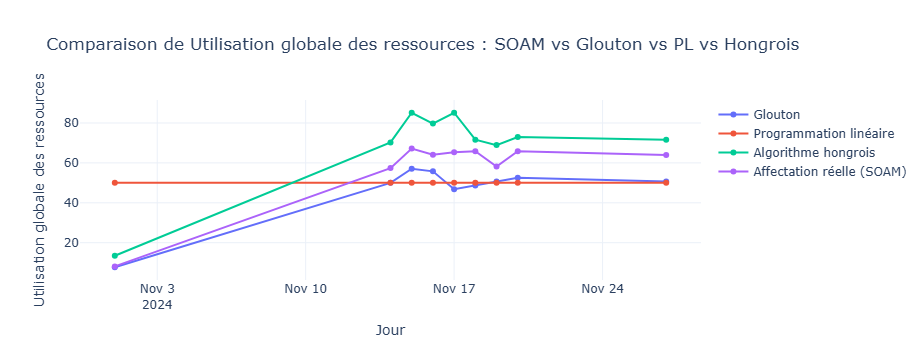
\includegraphics[width=0.8\linewidth]{assets/diagrams/overall_utilisation.png}
	\caption{Utilisation Globale des Ressources}
	\label{fig:overall_utilization}
\end{figure}


\begin{figure}[H]
	\centering
	\begin{minipage}{0.49\linewidth}
		\centering
		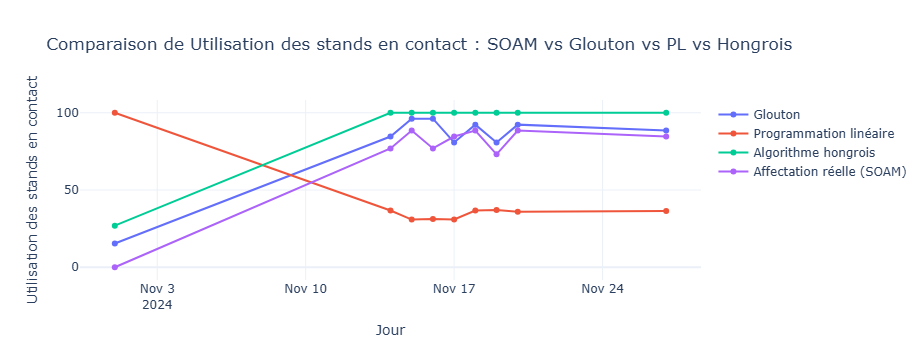
\includegraphics[width=\linewidth]{assets/diagrams/stand_contact.png}
		\caption{Utilisation des stands au contact}
		\label{fig:contact_utilization}
	\end{minipage}
	\hfill
	\begin{minipage}{0.49\linewidth}
		\centering
		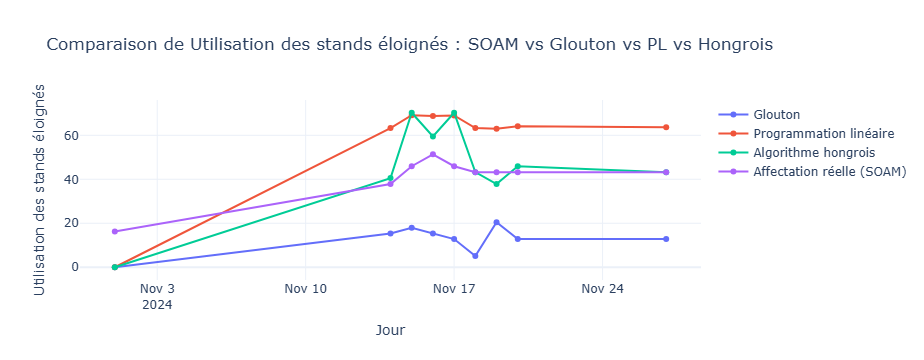
\includegraphics[width=\linewidth]{assets/diagrams/stand_eloigne.png}
		\caption{Utilisation des stands éloignés}
		\label{fig:remote_utilization}
	\end{minipage}
	\caption{Figure~\ref{fig:contact_and_remote}: Utilisation des stands de contact et des stands éloignés}
	\label{fig:contact_and_remote}
\end{figure}

\noindent
\textbf{Analyse :} D’après les figures, les approches algorithmiques – en particulier l’\textit{algorithme glouton} et l’\textit{algorithme hongrois} – surpassent nettement l’affectation réelle du \ac{SOAM} en maximisant l’utilisation des stands de contact. Ces méthodes permettent également une réduction notable de l’utilisation des stands éloignés, ce qui indique une meilleure efficacité des ressources. L’approche par \textit{programmation linéaire} performe également mieux que l’affectation réelle, mais reste en deçà des deux autres en termes d’utilisation optimale.

\paragraph{Répartition de l’Utilisation des Stands}

La figure~\ref{fig:stand_usage} montre la répartition des stands utilisés par terminal et type de vol (international vs. domestique), pour chaque méthode testée et l’affectation réelle.
\begin{figure}[H]
	\centering
	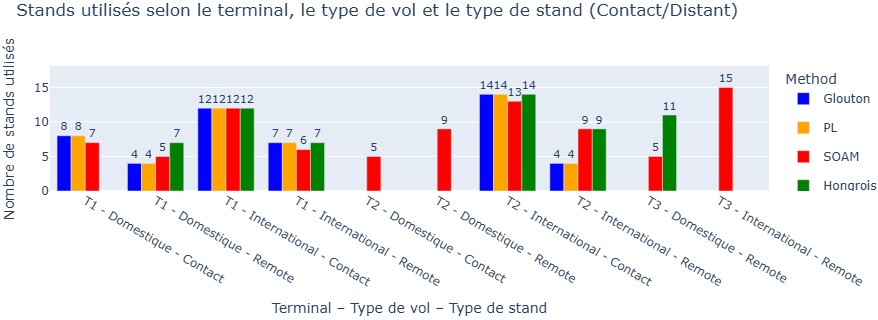
\includegraphics[width=1\textwidth]{assets/diagrams/terminal.jpg}
	\caption{Nombre de stands utilisés par terminal et type de vol selon les différents algorithmes et les affectations réelles.}
	\label{fig:stand_usage}
\end{figure}

\subsubsection{\textcolor{darkblue}{Comparaison Glouton vs. PL vs. Hongrois}}

Le tableau fournit une comparaison détaillée jour par jour en termes de temps d’exécution, coûts et métriques d’utilisation des ressources.
\begin{table}[htbp]
	\centering
	\caption{Comparaison des performances des algorithmes sur l’ensemble des jours de test}
	\label{tab:algorithm_comparison}
	\resizebox{\textwidth}{!}{%
		\begin{tabular}{|c|c|c|c|c|c|c|c|c|c|c|}
			\hline
			\multirow{2}{*}{\textbf{Jour}} & \multirow{2}{*}{\textbf{Vols}} & \multicolumn{3}{c|}{\textbf{Algorithme Hongrois}} & \multicolumn{3}{c|}{\textbf{Algorithme Glouton}} & \multicolumn{3}{c|}{\textbf{Programmation Linéaire}} \\
			\cline{3-11}
			& & \textbf{Temps (s)} & \textbf{Coût Total} & \textbf{Coût Moyen} & \textbf{Temps (s)} & \textbf{Coût Total} & \textbf{Coût Moyen} & \textbf{Temps (s)} & \textbf{Coût Total} & \textbf{Coût Moyen} \\
			\hline
			24-11-01 & 7 & 0.048 & \textbf{-280} & \textbf{-40.00} & \textbf{0.009} & \textbf{-280} & \textbf{-40.00} & 0.260 & \textbf{-280} & \textbf{-40.00} \\
			24-11-14 & 79 & \textbf{0.391} & -2000 & -25.31 & \textbf{0.126} & \textbf{-2420} & \textbf{-30.63} & 12.512 & -615 & -7.78 \\
			24-11-15 & 94 & \textbf{0.454} & -1715 & -18.24 & \textbf{0.172} & \textbf{-2960} & \textbf{-31.49} & 18.975 & -455 & -4.84 \\
			24-11-16 & 93 & 0.456 & -1835 & -19.73 & \textbf{0.156} & \textbf{-2465} & \textbf{-26.51} & 18.584 & -560 & -6.02 \\
			24-11-17 & 97 & 0.483 & -1730 & -17.83 & \textbf{0.153} & \textbf{-2935} & \textbf{-30.26} & 19.132 & -600 & -6.19 \\
			24-11-18 & 79 & 0.385 & -2050 & -25.63 & \textbf{0.151} & \textbf{-2775} & \textbf{-35.13} & 15.922 & -650 & -8.23 \\
			24-11-19 & 73 & 0.347 & -2095 & -28.69 & \textbf{0.099} & \textbf{-2115} & \textbf{-28.69} & 12.627 & -600 & -8.22 \\
			24-11-20 & 78 & 0.380 & -2040 & -26.15 & \textbf{0.128} & \textbf{-2535} & \textbf{-32.50} & 13.825 & -665 & -8.53 \\
			24-11-27 & 77 & 0.374 & -2040 & -26.49 & \textbf{0.114} & \textbf{-2515} & \textbf{-32.66} & 13.895 & -685 & -8.90 \\
			\hline
			\multicolumn{11}{|c|}{\textbf{Résumé de l’utilisation des ressources}} \\
			\hline
			\multicolumn{2}{|c|}{\textbf{Métrique}} & \multicolumn{3}{c|}{\textbf{Algorithme Hongrois}} & \multicolumn{3}{c|}{\textbf{Algorithme Glouton}} & \multicolumn{3}{c|}{\textbf{Programmation Linéaire}} \\
			\cline{3-11}
			\multicolumn{2}{|c|}{Util. Moyenne Stands Contact (\%)} & \multicolumn{3}{c|}{\textbf{91.88}} & \multicolumn{3}{c|}{84.73} & \multicolumn{3}{c|}{40.62} \\
			\multicolumn{2}{|c|}{Util. Moyenne Stands Distance (\%)} & \multicolumn{3}{c|}{\textbf{45.64}} & \multicolumn{3}{c|}{12.47} & \multicolumn{3}{c|}{62.37} \\
			\multicolumn{2}{|c|}{Taux d’Assignation (\%)} & \multicolumn{3}{c|}{\textbf{100}} & \multicolumn{3}{c|}{94} & \multicolumn{3}{c|}{\textbf{100}} \\
			\hline
		\end{tabular}
	}
\end{table}


L’évaluation expérimentale met en évidence les forces et limites de chaque algorithme. \textbf{L’algorithme hongrois} maximise l’usage des stands de contact (91{,}88\%), mais ne parvient pas à respecter tous les contraintes ( surtout la contrainte des stands incompatibles voir Annexe~\ref{tab:incompatibilites_stands}), en raison de sa contrainte de matrice carrée et de traitement par lot. \textbf{L’algorithme glouton} est le plus rapide (0{,}123s) et obtient les meilleurs coûts, mais son approche myope limite le taux d’affectation (94\%). \textbf{La programmation linéaire} assure une affectation complète (100\%) sans violation de contraintes, mais son temps d’exécution élevé (15{,}7s) réduit son applicabilité en temps réel.

Aucun algorithme ne présente un équilibre parfait entre efficacité, complétude d’affectation et utilisation des ressources. Ainsi, deux stratégies Hybridees sont proposées : une initialisation gloutonne rapide suivie d’un raffinement par algorithme génétique \ac{GA}, permettant de pallier les faiblesses individuelles tout en restant adaptée aux environnements dynamiques  et une autre combinant recuit simulé \ac{SA} et recherche tabou (TS), offrant une exploration efficace de l’espace des solutions avec un affinage local robuste.
\vspace{-1.7em}
\subsection{Comparaison Approfondie avec l’Affectation Réelle}

Cette section évalue les performances des approches hybrides combinant plusieurs stratégies d’optimisation.

\begin{itemize}
	\item Approche Hybridee Glouton+GA vs. Recuit simulé + Recherche tabou
	\item Comparaison avec les affectations réelles
\end{itemize}

\paragraph{Analyse de l’Utilisation des Ressources}

Les figures~\ref{fig:contact_and_remote_H} et~\ref{fig:overall_and_rate_H} comparent l’utilisation des stands (contact et éloignés) et la répartition des stands par terminal et type de vol.
\begin{figure}[H]
	\centering
	\begin{minipage}{0.49\linewidth}
		\centering
		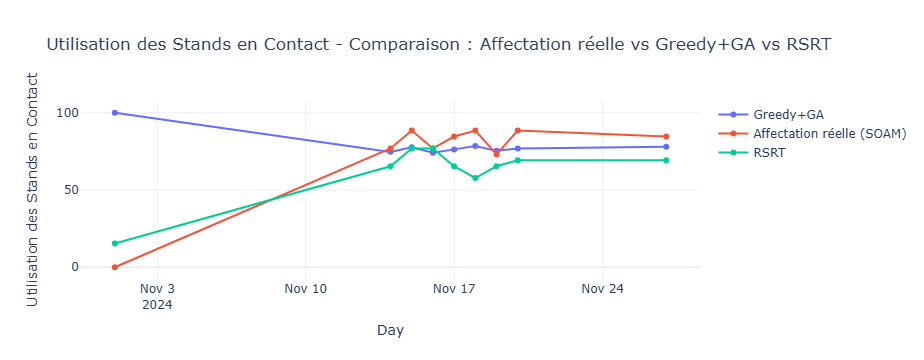
\includegraphics[width=\linewidth]{assets/diagrams/contactgasa.png}
		\caption{Utilisation des stands au contact
		}
		\label{fig:contact_utilization_H}
	\end{minipage}
	\hfill
	\begin{minipage}{0.49\linewidth}
		\centering
		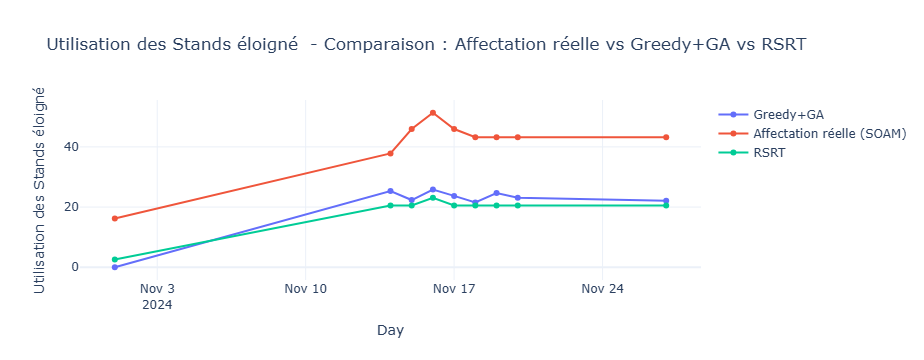
\includegraphics[width=\linewidth]{assets/diagrams/eloignegasa.png}
		\caption{Utilisation des stands éloignés
		}
		\label{fig:remote_utilization_H}
	\end{minipage}
	\caption{Figure~\ref{fig:contact_and_remote_H}: Utilisation des stands de contact et des stands éloignés.}
	\label{fig:contact_and_remote_H}
\end{figure}

\begin{figure}[H]
	\centering
	\begin{minipage}{0.49\linewidth}
		\centering
		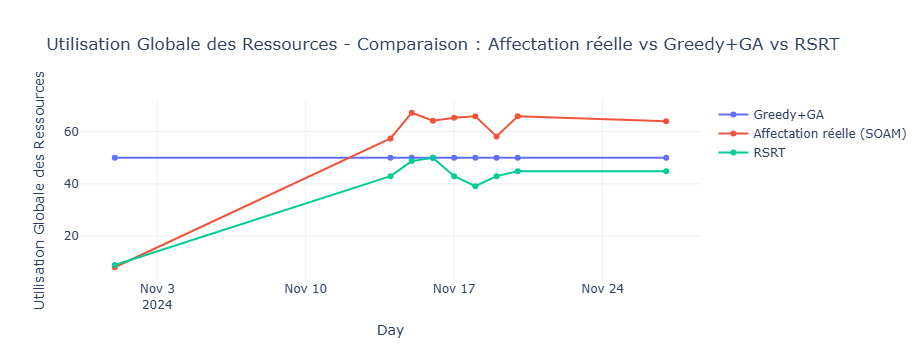
\includegraphics[width=\linewidth]{assets/diagrams/global_uti_gavssa.png}
		\caption{Utilisation globale des ressources}
		\label{fig:overall_utilization_H}
	\end{minipage}
	\hfill
	\begin{minipage}{0.49\linewidth}
		\centering
		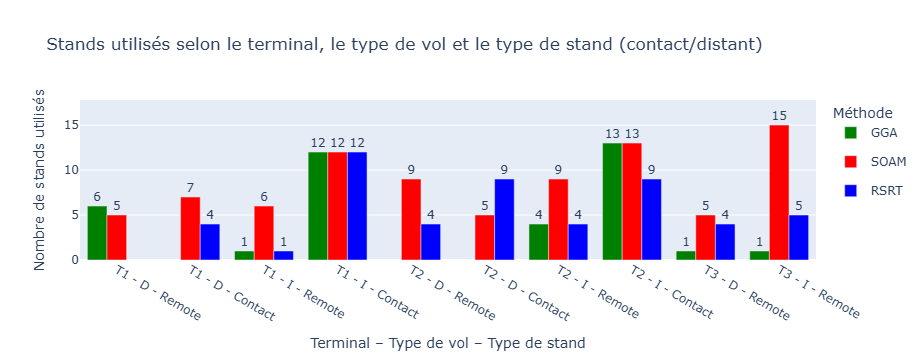
\includegraphics[width=\linewidth]{assets/diagrams/terminal_type.png}
		\caption{Taux d’affectation des vols}
		\label{fig:terminal_H}
	\end{minipage}
	\caption{Figure~\ref{fig:overall_and_rate_H}: Comparaison de l’utilisation globale et du taux d’affectation.}
	\label{fig:overall_and_rate_H}
\end{figure}


\subsubsection{Comparaison Glouton+GA vs. RSRT}

Le tableau~\ref{tab:RSRT_vs_gga} compare les performances de l’approche Hybridee Glouton + \ac{GA} et de l’approche Hybridee Recuit simulé + Recherche tabou .
\begin{table}[htbp]
	\centering
	\caption{Comparaison des performances : RSRT vs. Hybride Glouton+AG}
	\label{tab:RSRT_vs_gga}
	\resizebox{\textwidth}{!}{%
		\begin{tabular}{|c|c|c|c|c|c|c|c|}
			\hline
			\multirow{2}{*}{\textbf{Jour}} & \multirow{2}{*}{\textbf{Vols}} 
			& \multicolumn{3}{c|}{\textbf{RSRT (Recuit simulé + Recherche tabou)}} 
			& \multicolumn{3}{c|}{\textbf{Hybride Glouton+AG}} \\
			\cline{3-8}
			& & \textbf{Coût Total} & \textbf{Coût Moyen} & \textbf{Temps exéc. (s)} 
			& \textbf{Coût Total} & \textbf{Coût Moyen} & \textbf{Temps exéc. (s)} \\
			\hline
			01-11-2024 & 7  & -280   & -40.00  & 0.87       & \textbf{-2030}   & \textbf{-290.00}  & 0.4648 \\
			14-11-2024 & 79 & -2420  & -30.63  & 24.52      & \textbf{-195130} & \textbf{-2470.00} & 5.2960 \\
			15-11-2024 & 94 & -2960  & -31.49  & 25.39      & \textbf{-279650} & \textbf{-2975.00} & 6.7000 \\
			16-11-2024 & 93 & -2465  & -26.51  & 403.01     & \textbf{-273420} & \textbf{-2940.00} & 6.6312 \\
			17-11-2024 & 97 & -2935  & -30.26  & 35.37      & \textbf{-291000} & \textbf{-3000.00} & 7.3665 \\
			18-11-2024 & 79 & -2775  & -35.13  & 23.59      & \textbf{-201055} & \textbf{-2545.00} & 5.5957 \\
			19-11-2024 & 73 & -2115  & -28.97  & 28.26      & \textbf{-174105} & \textbf{-2385.00} & 4.9329 \\
			20-11-2024 & 78 & -2535  & -32.50  & 24.20      & \textbf{-198120} & \textbf{-2540.00} & 5.5983 \\
			27-11-2024 & 77 & -2515  & -32.66  & 20.09      & \textbf{-187110} & \textbf{-2430.00} & 5.3974 \\
			\hline
			\multicolumn{8}{|c|}{\textbf{Résumé de l’utilisation des ressources}} \\
			\hline
			\multicolumn{2}{|c|}{\textbf{Métrique}} 
			& \multicolumn{3}{c|}{\textbf{RSRT (Recuit simulé + Recherche tabou)}} 
			& \multicolumn{3}{c|}{\textbf{Hybride Glouton+AG}} \\
			\hline
			\multicolumn{2}{|c|}{Utilisation moyenne des stands contact (\%)} 
			& \multicolumn{3}{c|}{\textbf{69.43}} 
			& \multicolumn{3}{c|}{\textbf{76.83}} \\
			\multicolumn{2}{|c|}{Utilisation moyenne des stands distants (\%)} 
			& \multicolumn{3}{c|}{\textbf{18.76}} 
			& \multicolumn{3}{c|}{\textbf{22.06}} \\
			\multicolumn{2}{|c|}{Temps d’exécution moyen (s)} 
			& \multicolumn{3}{c|}{\textbf{65.71}} 
			& \multicolumn{3}{c|}{\textbf{5.33}} \\
			\hline
		\end{tabular}
	}
\end{table}

\section{Interprétation des résultats et justification du choix de l’algorithme}

L’analyse comparative entre l’algorithme RSRT (Recuit simulé + Recherche tabou) et l’algorithme Hybride Glouton+GA (GGA) met en évidence plusieurs points clés.

\subsection{Priorité à l’utilisation des stands contact}

L’utilisation moyenne des stands contact, qui représentent une ressource prioritaire pour le traitement rapide et efficace des vols, est significativement plus élevée avec GGA (76,83\,\%) qu’avec RSRT (69,43\,\%). Cette optimisation reflète la capacité de GGA à mieux respecter la priorité accordée aux stands contact par rapport aux stands distants, favorisant ainsi une meilleure qualité de service.

\subsection{Coût total et coût moyen}

Les résultats montrent que GGA permet d’obtenir des coûts totaux et moyens nettement inférieurs, traduisant une meilleure optimisation économique. Les coûts moyens tournent autour de -2500 pour GGA, contre environ -30 pour RSRT, ce qui souligne l’efficacité accrue de GGA dans l’affectation des ressources.

\subsection{Temps d’exécution}

Le temps d’exécution moyen de GGA est de 5,33 secondes, largement inférieur à celui de RSRT, qui est de 65,71 secondes. Cette différence est particulièrement importante dans un contexte opérationnel où la rapidité de prise de décision est essentielle. De plus, RSRT présente des pics de temps d’exécution très élevés, ce qui peut limiter son utilisation en temps réel.

\subsection{Justification du choix de l’algorithme Hybride Glouton + GA}

Compte tenu de ces résultats, l’algorithme Hybride Glouton + GA constitue un compromis optimal entre qualité de solution et efficacité temporelle. Il permet de :

\begin{itemize}
	\item Réduire significativement les coûts opérationnels,
	\item Respecter les priorités d’utilisation des stands, en maximisant l’utilisation des stands contact,
	\item Garantir un temps de calcul réduit, adapté à un environnement aéroportuaire dynamique nécessitant des décisions rapides.
\end{itemize}

Ainsi, GGA est la solution recommandée pour la gestion efficace des stands aéroportuaires, conciliant optimisation économique, respect des contraintes opérationnelles et performance temporelle. \textbf{Cette méthode sera adoptée pour son intégration avec l’interface Digital Twin, afin d’assurer une gestion en temps quasi-réel et optimisée des ressources aéroportuaires.}

\vspace{-1.3em}
\section{Intégration du modèle}
\vspace{-1em}
\subsection*{Informations Générales}
\begin{itemize}
	\item \textbf{Environnement :} \url{http://localhost:8000}
	\item \textbf{Date des tests :} \textcolor{darkblue}{16-06-2025}
	\item \textbf{Outils Utilisés :} \textcolor{darkblue}{FastAPI, Swagger UI}
	\item \textbf{Base de données :}\textcolor{darkblue}{ Fichiers CSV (\texttt{all\_flights.csv}, \texttt{stand.csv})}
	
\end{itemize}
\vspace{0.15cm}
Cette API permet de faire l'affectation des vols aux stands disponibles dans un aéroport en fonction de diverses contraintes et paramètres.Les principaux objectifs de cette évaluation sont :
\begin{itemize}
	\item La performance et le temps de réponse de l'API
	\item La gestion des erreurs et des cas limites :
	\begin{itemize}
		\item Évaluer comment l'API gère les erreurs en cas de saisie incorrecte, de champs manquants ou de valeurs non valides
		\item Assurer que des messages d'erreur clairs et appropriés sont retournés
	\end{itemize}
\end{itemize}

\vspace{-1.3em}
\subsection*{Méthodologie de Test}
Cette partie décrit la méthodologie utilisée pour tester les fonctionnalités de l’API.
\vspace{-1em}
\subsubsection{Entrées du système}

\fcolorbox{black!20}{gray!5}{
	\begin{minipage}{\linewidth}
		\texttt{\textcolor{darkblue}{\{}}\\
		\hspace*{1em}\texttt{\textcolor{darkblue}{"date": "2024-11-01",}}\\
		\hspace*{1em}\texttt{\textcolor{darkblue}{"start\_time": "08:00",}}\\
		\hspace*{1em}\texttt{\textcolor{darkblue}{"end\_time": "18:00"}}\\
		\texttt{\textcolor{darkblue}{\}}}
	\end{minipage}
}
\vspace{0.15cm}

\begin{itemize}
	\item \textbf{date} : La date pour laquelle l’affectation doit être réalisée, au format \texttt{YY-MM-DD} (ISO)
	\item \textbf{start\_time} : Heure de début de la plage horaire au format 24h (\texttt{HH:MM})
	\item \textbf{end\_time} : Heure de fin de la plage horaire au format 24h (\texttt{HH:MM})
\end{itemize}
\vspace{-0.5em}
\subsubsection{Tests fonctionnels des endpoints}
\vspace{-0.7em}
Le tableau~\ref{tab:tests-endpoints} présente une série de tests effectués sur les différents endpoints de l’API. Chaque requête est testée pour valider la réponse attendue, tant sur le contenu que sur le format.
\vspace{-1em}
\begin{table}[H]
	\centering
	\renewcommand{\arraystretch}{0.6}
	\caption{Tests fonctionnels des endpoints principaux de l’API}
	\begin{tabularx}{\textwidth}{p{3.3cm} p{3.5cm} p{3.5cm} p{4.6cm}}
		\toprule
		\textbf{Endpoint} & \textbf{Description} & \textbf{Résultat attendu} & \textbf{Résultat obtenu} \\
		\midrule
		\texttt{GET /} &
		Vérification de la racine de l'API &
		Message de bienvenue &
		\texttt{\{"message": "Welcome to Airport Stand Assignment API"\}} \\
		
		\midrule
		\texttt{GET /available-dates/} &
		Récupération des dates disponibles &
		Liste des dates contenues&
		Liste correctement reçue \\
		
		\midrule
		\texttt{POST /assign-stands/} &
		Affectation des vols pour une journée &
		Résultat JSON avec durée de traitement &
		Réponse structurée avec les données affectées \\
		
		\bottomrule
	\end{tabularx}
	\label{tab:tests-endpoints}
\end{table}

\vspace{-1.7em}


\subsubsection{Tests de performance}

Pour une évaluation approfondie, trois journées aux trafics variés ont été choisies afin de tester le système dans différentes conditions:
\begin{itemize}
	\item nombre de vols minimal \textcolor{darkblue}{(jour avec seulement 1 vol)},
	\item nombre de vols moyen \textcolor{darkblue}{(jour avec 70 vols)},
	\item nombre de vols maximal \textcolor{darkblue}{(jour avec 97 vols)}.
\end{itemize}

Les tests ont été exécutés sur l'ensemble de la journée \textcolor{darkblue}{(de 00:00 à 23:59)} afin de capturer toutes les variations possibles de performance selon les plages horaires.

Le tableau~\ref{tab:tests-performance} résume les résultats obtenus, avec le temps de réponse mesuré pour chaque cas.

\begin{table}[H]
	\centering
	\renewcommand{\arraystretch}{0.9}
	\caption{Performance de l’API en fonction du volume de vols à traiter}
	\begin{tabularx}{\textwidth}{l l l X X}
		\toprule
		\textbf{Date} & \textbf{Heure début} & \textbf{Heure fin} & \textbf{Nombre de vols} & \textbf{Temps de réponse (s)} \\
		\midrule
		24-11-03 & 00:00 & 23:59 & 1 & Pas d'affectation \\
		24-11-01 & 00:00 & 23:59 & 8 & 0.95 \\
		24-11-12 & 00:00 & 23:59 & 70 & 4.95 \\
		24-11-17 & 00:00 & 23:59 & 97 & 8.05 \\
		\bottomrule
	\end{tabularx}
	\label{tab:tests-performance}
\end{table}

\noindent
\textit{Remarque :} Lorsqu'une seule rotation est enregistrée dans une journée, aucune affectation de stand n’est effectuée, car aucune succession n’est possible.

\subsubsection{Tests de validation et gestion des erreurs}
Le tableau~\ref{tab:erreurs-api} illustre une série de cas de test validant la gestion des erreurs par l'API. Il couvre généralement les principaux cas limites.
\vspace{-1em}
\begin{table}[H]
	\centering
	\renewcommand{\arraystretch}{0.5}
	\caption{Exemples de scénarios d'erreurs et messages retournés par l'API}
	\vspace{-0.5em}
	\begin{tabularx}{\textwidth}{l X X}
		\toprule
		\textbf{Scénario} & \textbf{Données en entrée} & \textbf{Message retourné} \\
		\midrule
		Format de date invalide &
		\texttt{\{"date": "14-11-2024", "start\_time": "08:00", "end\_time": "18:00"\}} &
		Format de date invalide. Utilisez le format AA-MM-JJ \textcolor{darkblue}{(ex: 24-11-14)}. \\
		
		\midrule
		Format d'heure invalide &
		\texttt{\{"date": "24-11-14", "start\_time": "8h00", "end\_time": "18:00"\}} &
		Le format de l'heure doit être HH:MM en 24h \textcolor{darkblue}{(ex: 14:30)}. \\
		
		\midrule
		Dates hors plage &
		\texttt{\{"date": "24-10-01", "start\_time": "08:00", "end\_time": "18:00"\}} &
		Les dates suivantes ne sont pas présentes dans le jeu de données : \textcolor{darkblue}{24-10-01}. \\
		
		\midrule
		Date manquante &
		\texttt{\{"date": " ", "start\_time": "08:00", "end\_time": "18:00"\}} &
		La date ne peut pas être vide. \\
		
		\midrule
		Mois invalide &
		\texttt{\{"date": "24-13-01", "start\_time": "08:00", "end\_time": "18:00"\}} &
		Le mois doit être entre 01 et 12, reçu 13. \\
		
		\midrule
		Jour invalide &
		\texttt{\{"date": "24-10-40", "start\_time": "08:00", "end\_time": "18:00"\}} &
		Le jour doit être entre 01 et 31, reçu 40. \\
		
		\midrule
		Heure de début > heure de fin &
		\texttt{\{"date": "24-11-14", "start\_time": "18:00", "end\_time": "08:00"\}} &
		L'heure de début doit être antérieure à l'heure de fin. \\
		
		\bottomrule
	\end{tabularx}
	\label{tab:erreurs-api}
\end{table}


\subsection*{Mécanismes internes du système}

Le système repose sur deux mécanismes clés pour optimiser le traitement.

\begin{itemize}
	\item \textbf{Mécanisme de mise en cache :} Réutilisation directe des résultats précédemment calculés.
	\item \textbf{Traitement temporel :} Affectation journalière suivie d’un filtrage par intervalle.
\end{itemize}
\vspace{-1.5em}
\subsection{Qualité des affectations}

Le tableau~\ref{tab:qualite-affectations} évalue la qualité des affectations pour trois journées à fort trafic, en indiquant la répartition des types de stands et le taux de compatibilité avion/stand.

\begin{table}[H]
	\centering
	\renewcommand{\arraystretch}{1}
	\caption{Qualité des affectations par date : répartition des stands et compatibilité}
	\begin{tabularx}{\textwidth}{l c c c c}
		\toprule
		\textbf{Date} & \textbf{Nb. de vols} & \textbf{Stands Contact} & \textbf{Stands Remote} & \textbf{Compatibilité avion/stand} \\
		\midrule
		24-11-12 & 70 & 18 & 7 & 100\% \\
		24-11-14 & 80 & 20 & 8 & 100\% \\
		24-11-17 & 97 & 16 & 14 & 100\% \\
		\bottomrule
	\end{tabularx}
	\label{tab:qualite-affectations}
\end{table}


\textbf{Chevauchement temporel :} Aucun



L’algorithme d’affectation génère un fichier au format JSON, où chaque vol est associé à un stand en fonction des contraintes opérationnelles et physiques. Un extrait représentatif de ce fichier est présenté ci-dessous.

L’intégralité du résultat d’affectation pour les journées testées est fournie en annexe, accompagnée de la signification de chaque attribut utilisé dans le fichier (cf. Table~\ref{tab:attributs_vols_complet}).

L’API respecte les objectifs fonctionnels fixés. L’algorithme propose des affectations pertinentes, conformes aux contraintes, avec une répartition équilibrée entre stands de contact et éloignés, et un taux de compatibilité avion/stand satisfaisant. 


\section{Réalisation}
Cette section présente les interfaces principales de l'application développée.

\subsection*{Visualisation des indicateurs de performance (KPI)}

Cette capture d'ecran presente 
L’interface développée intègre une section dédiée à la visualisation des \textbf{indicateurs de performance clés} (KPI), permettant de suivre et d’analyser en temps réel l’efficacité opérationnelle de l’affectation des stands avion.

L’image ci-dessous illustre cette interface de pilotage. Chaque encart correspond à un indicateur spécifique, calculé selon des règles métiers définies avec le client. Ces indicateurs ont pour objectif d’aider les décideurs à mieux comprendre l’utilisation des ressources, à identifier les retards ou anomalies, et à prendre des mesures correctives en cas de besoin.
\begin{figure}[H]
	\centering
	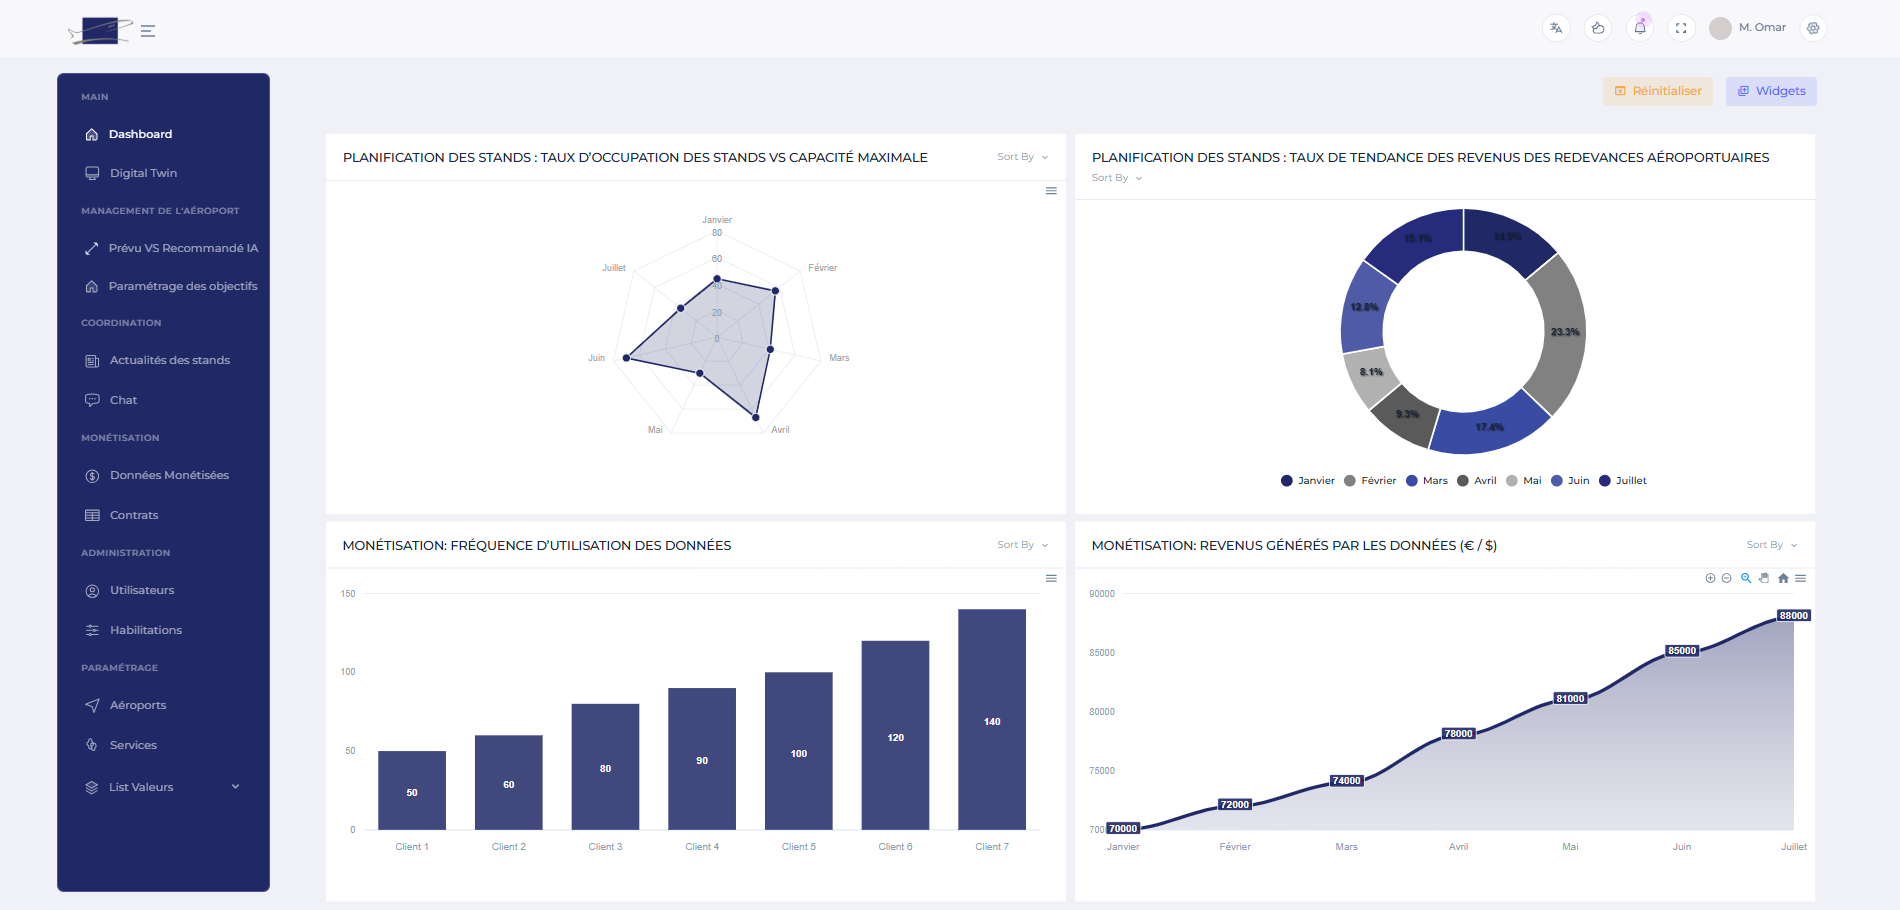
\includegraphics[width=0.95\textwidth]{assets/interfaces/kpi.png} % remplace par ton nom de fichier
	\caption{Interface de visualisation des KPI}
	\label{fig:kpi_interface}
\end{figure}

\subsection*{Fonctionnalité de recherche d’avion ou de stand}

L’une des fonctionnalités du jumeau numérique est la \textbf{recherche d’un avion ou d’un stand}, dans lequel l’utilisateur peut saisir : \textit{un matricule d’avion} ou \textit{un numéro de stand}


\begin{figure}[H]
	\centering
	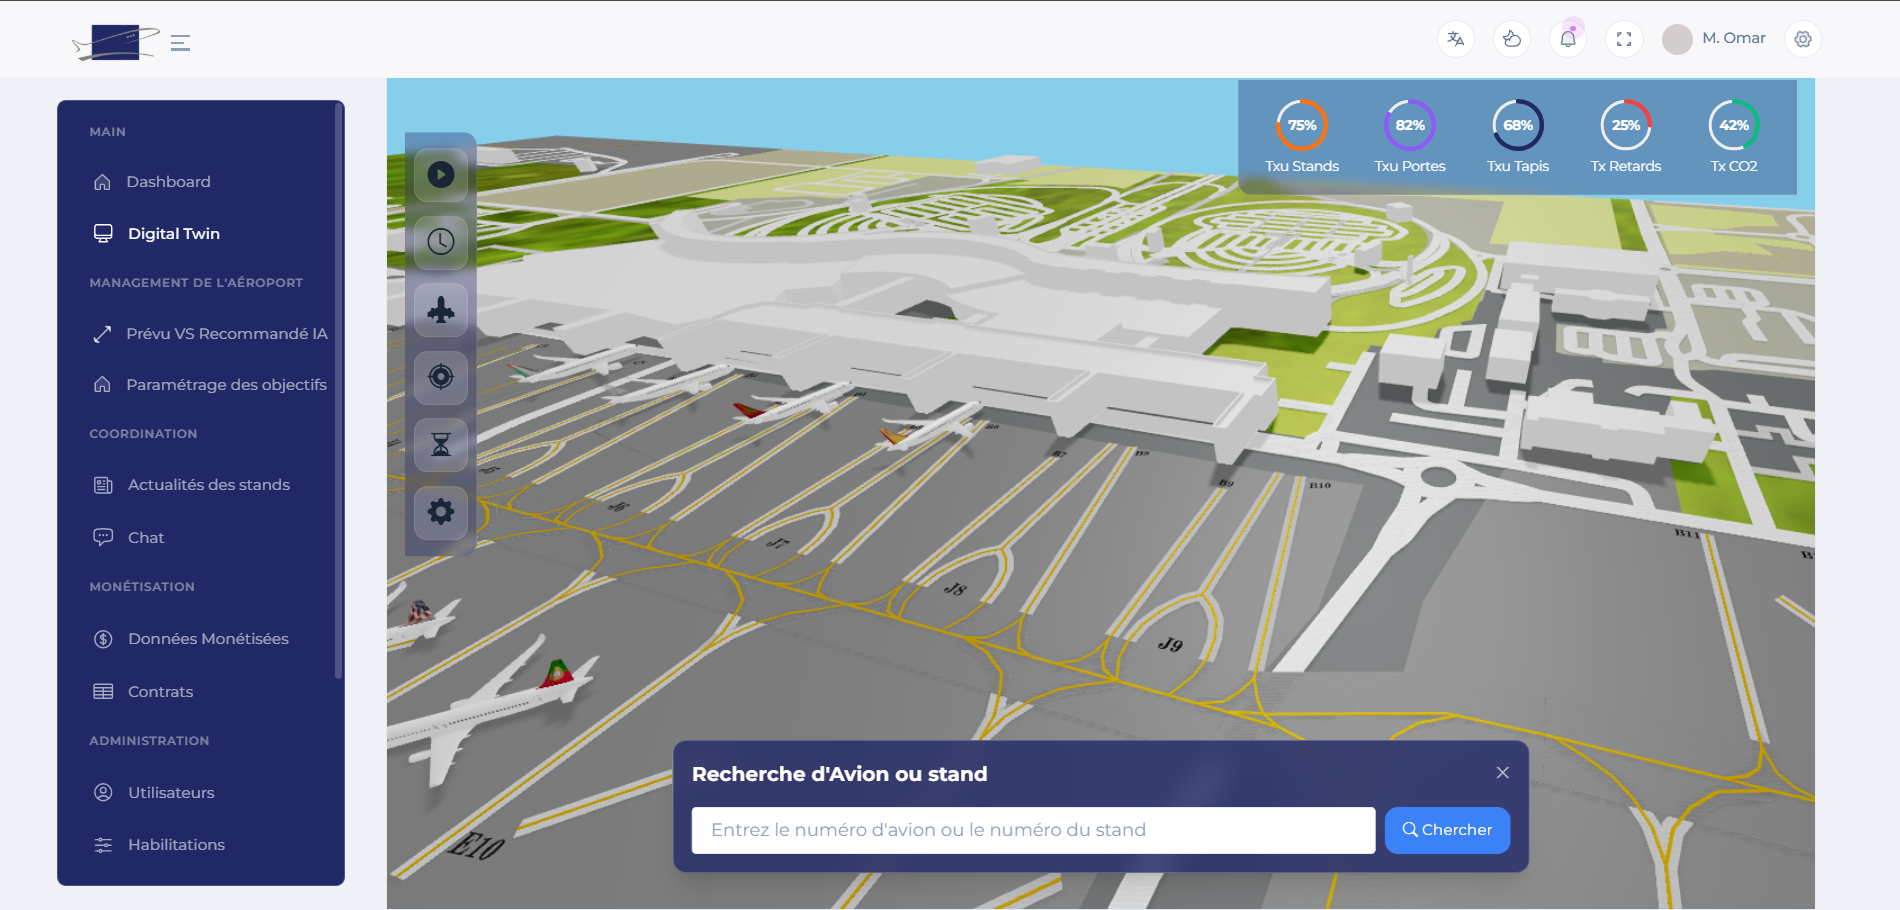
\includegraphics[width=0.95\textwidth]{assets/interfaces/recherche.png}
	\caption{Recherche d’un avion ou d’un stand avec affichage d’informations contextuelles}
	\label{fig:search_avion_stand}
\end{figure}
Une fois la recherche lancée, le système effectue une requête interne qui recentre automatiquement la vue 3D sur l’objet ciblé (avion ou stand) et affiche une fiche d’information contextuelle contenant plusieurs détails : matricule de l’avion, numéro du stand, statut du vol (ex.~: À l’heure), compagnie aérienne (ex.~: Spain Air), provenance (ex.~: New York (JFK)), marque de l’avion (ex.~: Airbus) et nombre de passagers (ex.~: 220).
\begin{figure}[H]
	\centering
	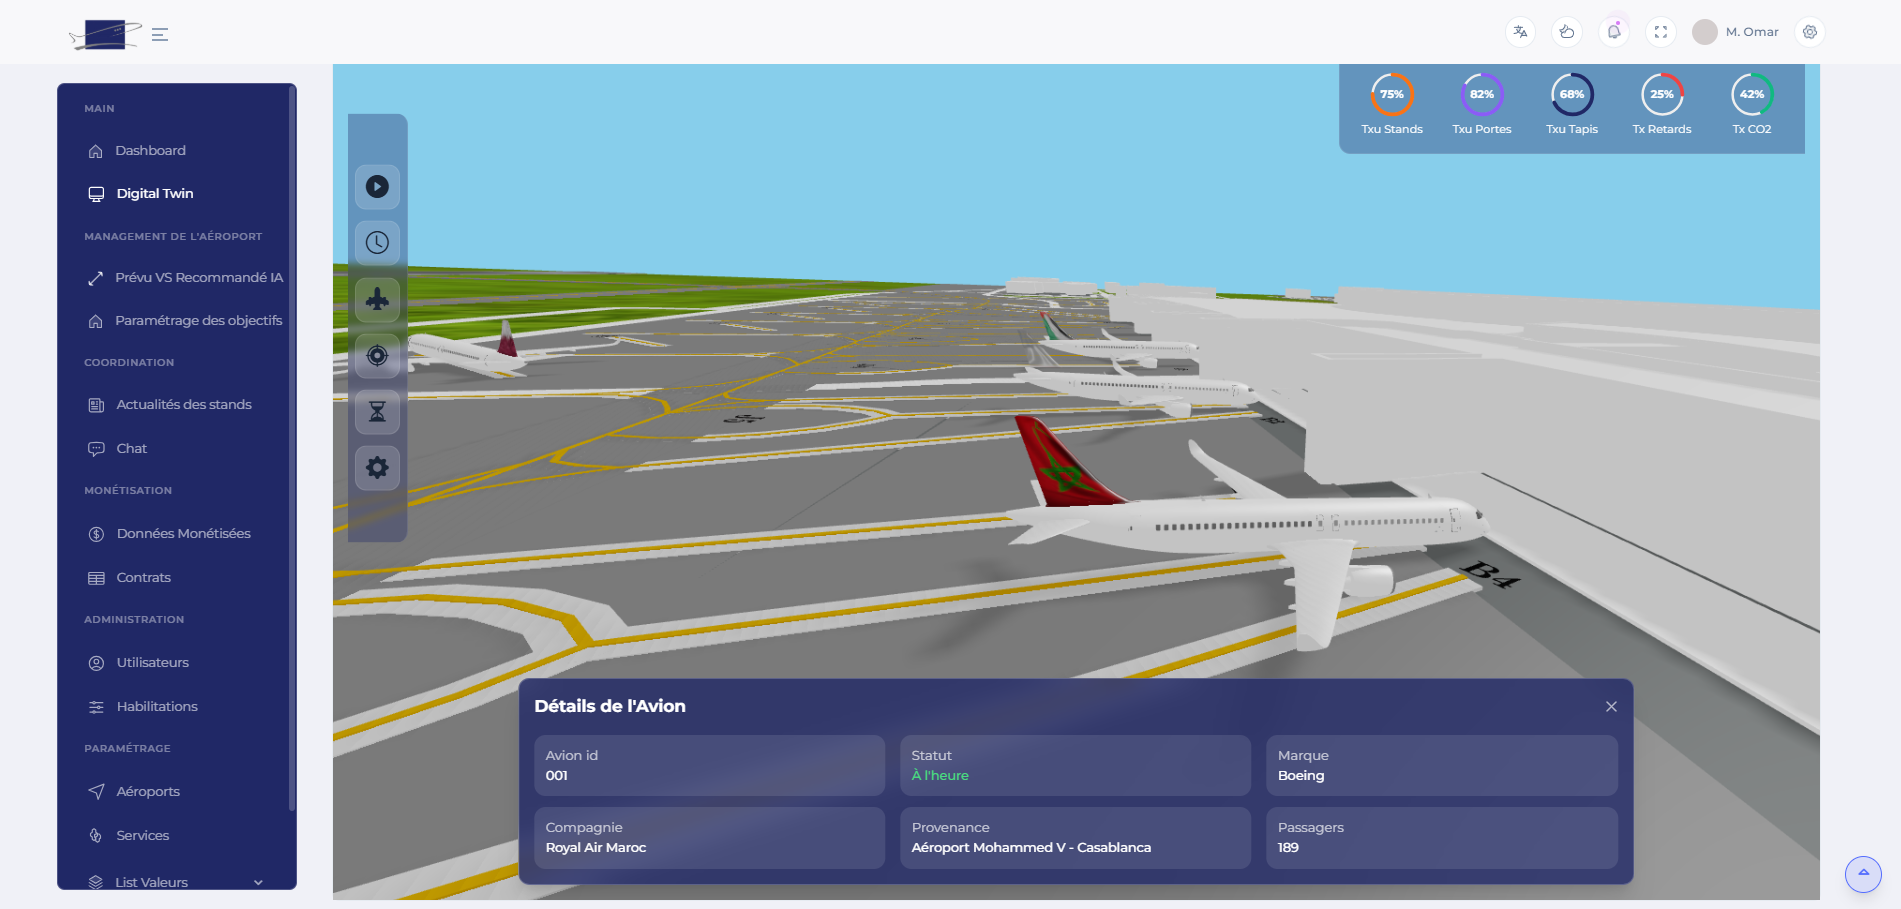
\includegraphics[width=0.85\textwidth]{assets/interfaces/affichageRecherche.png} % Remplace par ton image réelle
	\caption{Recherche d’un avion ou d’un stand avec affichage d’informations contextuelles}
	\label{fig:search_avion_stand}
\end{figure}

\subsection*{Simulation d’une journée d’activité passée}

L’interface du jumeau numérique permet aux utilisateurs de \textbf{simuler une journée d’activité antérieure} afin d’analyser le déroulement des opérations passées, détecter d’éventuelles anomalies, et évaluer la performance globale de l’aéroport.

Cette fonctionnalité se déroule en plusieurs étapes illustrées ci-dessous :

\begin{enumerate}
	\item \textbf{Sélection de la plage horaire}~: l’utilisateur choisit une date et une plage horaire. 
	\begin{figure}[H]
		\centering
		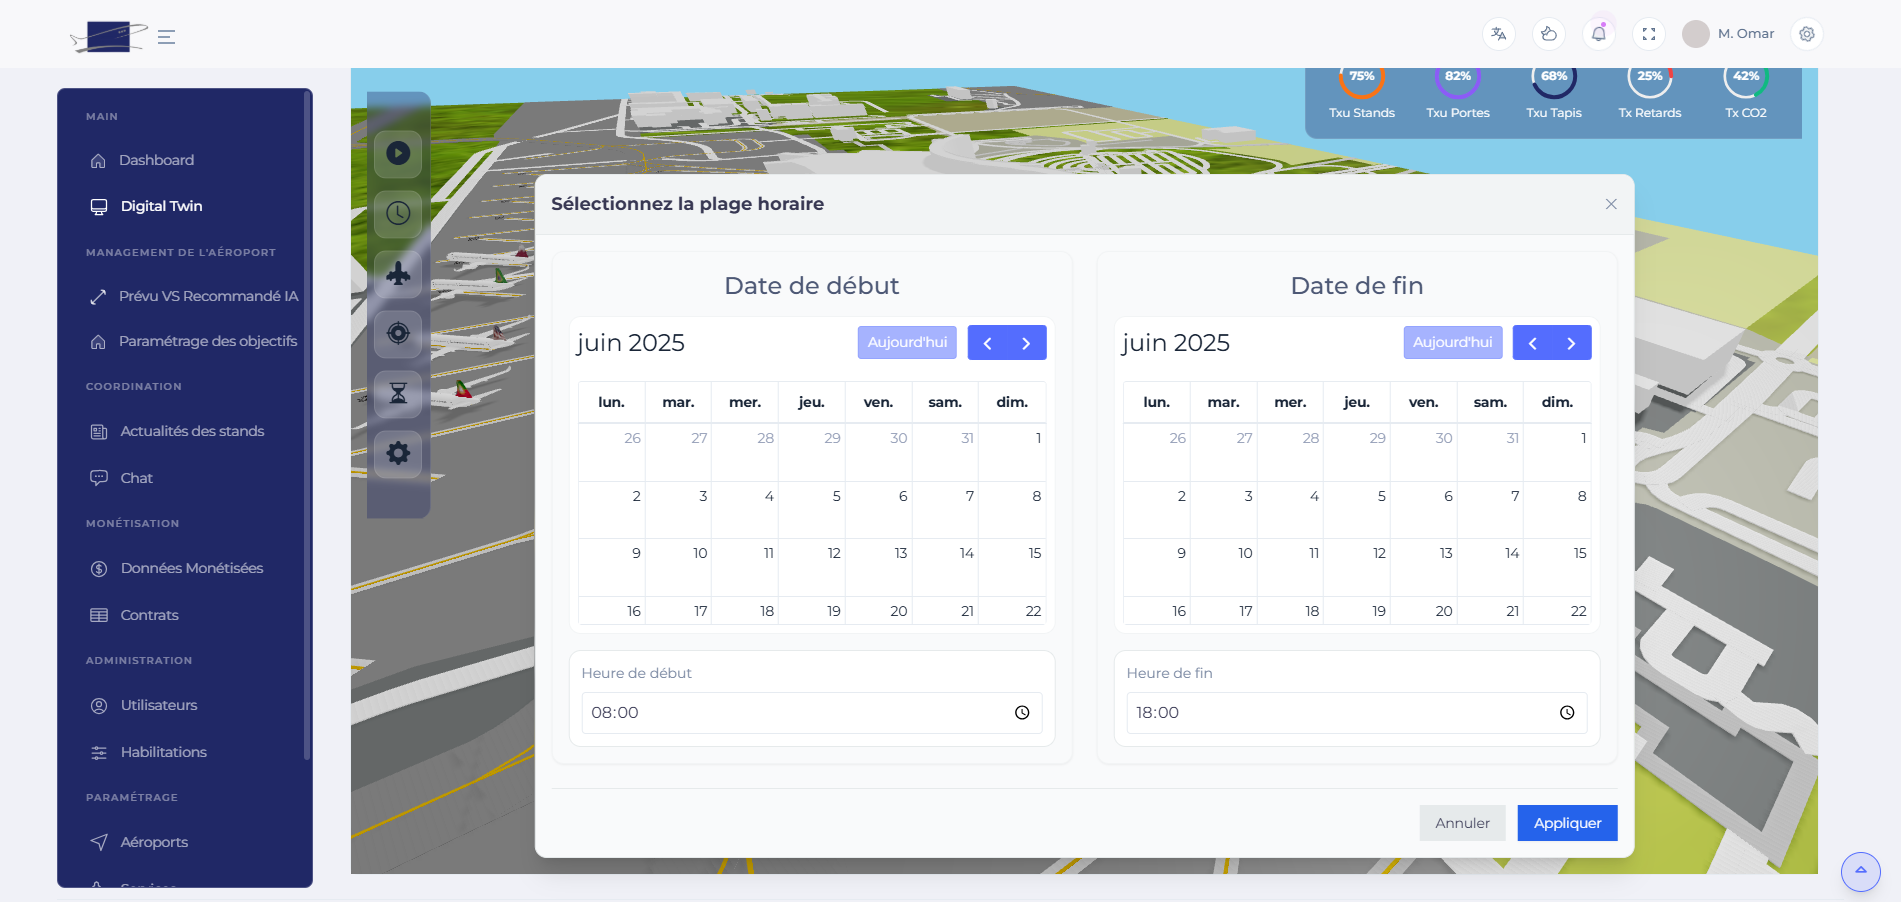
\includegraphics[width=0.95\textwidth]{assets/interfaces/simulation.png}
		\caption{Choix de la plage horaire pour la simulation d'une journée passée}
		\label{fig:simulation1}
	\end{figure}
	
	\item \textbf{Lancement de la simulation}~: une fois les paramètres validés, le système informe l’utilisateur que la simulation est en cours d’exécution.

	
	\item \textbf{Lecture de la simulation}~: l’activité de l’aéroport s’anime dans l’interface 3D sous forme de lecture chronologique. L’utilisateur peut ainsi visualiser l’évolution des vols, les affectations aux stands, les retards, les conflits, ou les événements inattendus.
	

\end{enumerate}

Cette fonctionnalité constitue un outil d’analyse puissant, permettant de \textbf{rejouer des scénarios passés} pour mieux comprendre les dysfonctionnements.
\subsection*{Mise à jour de la planification recommandée}

L’interface du jumeau numérique permet de comparer deux niveaux de planification~:

\begin{itemize}
	\item \textbf{L’affectation prévisionnelle}~: il s’agit de la planification effective des vols et des ressources réalisée par le \ac{SOAM}.
	
	\item \textbf{La planification recommandée}~: elle est générée dynamiquement par le moteur d’optimisation.
\end{itemize}

Une interface dédiée permet aux utilisateurs de visualiser ces deux plannings côte à côte, facilitant ainsi l’analyse des écarts entre le scénario initial et la recommandation opérationnelle.
\begin{figure}[H]
	\centering
	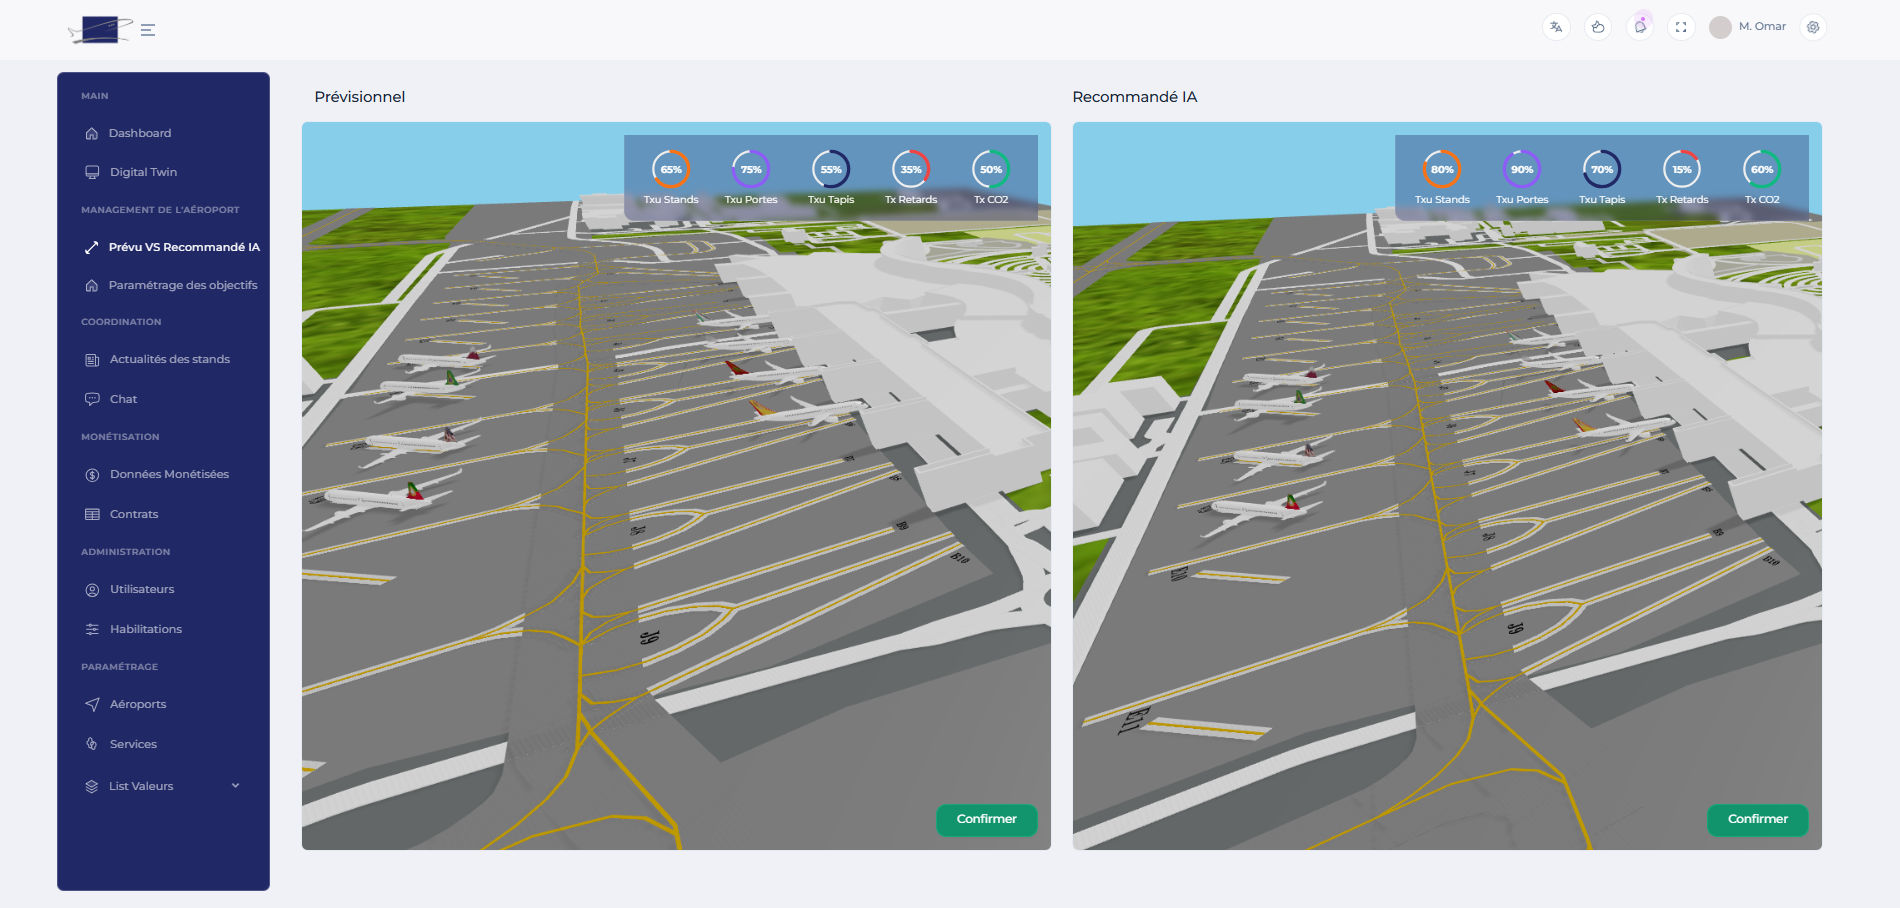
\includegraphics[width=0.95\textwidth]{assets/interfaces/comparaison.png} % Remplacer par ton image réelle
	\caption{Comparaison entre planification prévisionnelle et recommandée dans l’interface}
	\label{fig:planning_comparaison}
\end{figure}

\subsubsection*{Fonctionnalité 4 : Alertes et notifications}

L’interface dédiée au coordinateur intègre un système d’alertes et de notifications permettant d’améliorer la réactivité face aux événements critiques ou aux anomalies.

\begin{figure}[H]
	\centering
	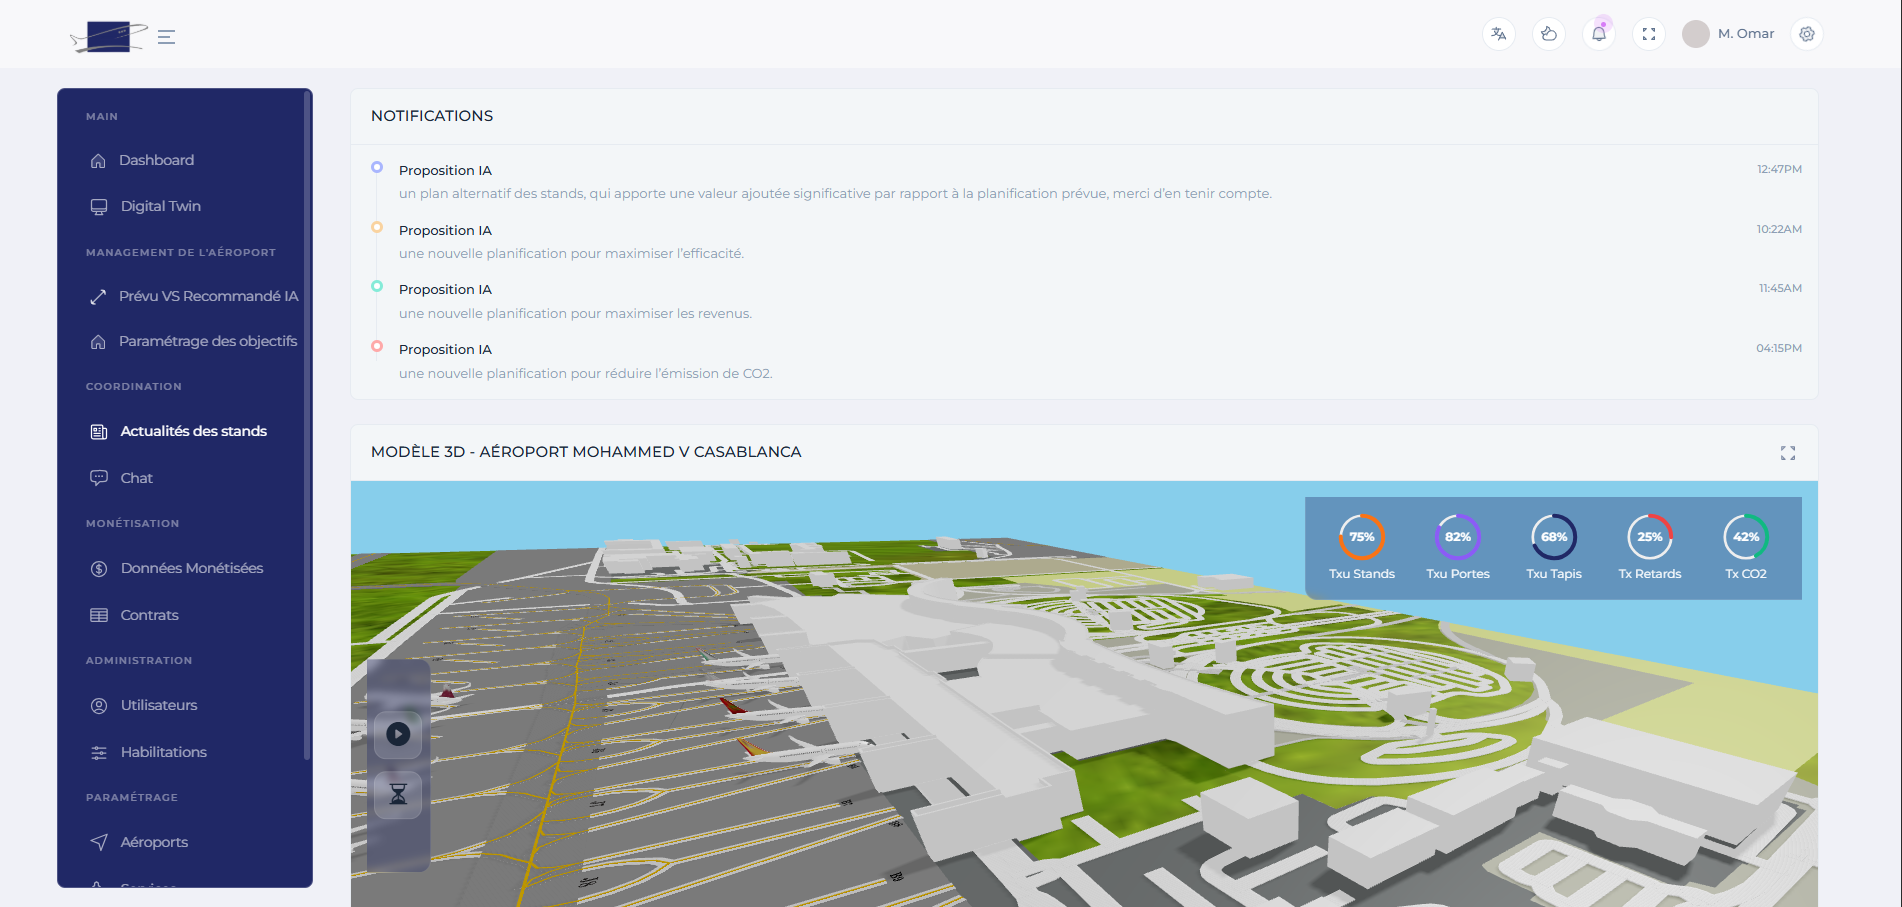
\includegraphics[width=0.95\textwidth]{assets/interfaces/alerte.png} % Remplace par ton image de notification
	\caption{Interface coordinateur : exemple d’alerte en cas de retard critique}
	\label{fig:alertes_notifications}
\end{figure}


\section{Conclusion}

Ce chapitre a présenté l’implémentation et le déploiement de notre solution d’affectation dynamique des stands. Après avoir défini les métriques d’évaluation, plusieurs approches algorithmiques ont été testées, dont le recuit simulé, la recherche tabou, l’algorithme glouton et l’algorithme génétique.

Les résultats ont montré que la combinaison de l’approche gloutonne et de l’algorithme génétique permet d’obtenir un bon équilibre entre coût, occupation optimale des stands contact et temps d’exécution. Cette approche hybride a donc été retenue comme module final du système.

Le modèle a été intégré dans une architecture complète, avec une interface de simulation, fournissant ainsi un outil intelligent d’aide à la décision adapté aux contraintes du domaine aéroportuaire.

